\begin{frame}{Forced oscillation}
\framesubtitle{Resonance curve}
\begin{figure}[ht]
   		\begin{tikzpicture}
   		\begin{axis}[
   		width=\linewidth,height=7cm,
   		title={Amplitude of forced oscillations as a function of angular frequency},
   		xlabel={Angular frequency / $s^{-1}$},
   		ylabel={Amplitude / arbitrary units},
   		xmajorgrids=true,ymajorgrids=true,
   		grid style=dashed,
   		]
   		
   		\addplot[smooth, solid,	color=blue,	mark=+,
   		mark options={solid,scale=2,line width=1.5pt}]		
   		table[x index = {3}, y index = {6}, col sep=comma]
   		{data/forced_oscillations_0.3A.csv};
   		\addlegendentry{braking current = \SI{0.3}{\ampere}}
   		\addplot [color=green,opacity=0.4, mark=*, mark size=5pt, forget plot] 
   		coordinates {(3.11,11.5)};
   		\draw [dashed,thick, color=black] (axis cs: -10,11.5) -| (axis cs: 3.11,-10);
   		
   		
   		\addplot[smooth, solid,	color=orange,	mark=+,
   		mark options={solid,scale=2,line width=1.5pt},
   		]		
   		table[x index = {3}, y index = {6}, col sep=comma]
   		{data/forced_oscillations_0.6A.csv};
   		\addlegendentry{braking current = \SI{0.6}{\ampere}}
   		\addplot [color=green,opacity=0.4, mark=*, mark size=5pt, forget plot] 
   		coordinates {(3.05,3.3)};
   		\draw [dashed,thick, color=black] (axis cs: -10,3.3) -| (axis cs: 3.05,-10);
   		
   		\end{axis}
   		\end{tikzpicture}
   		\label{fig:resonance-curve}
   	\end{figure}
\end{frame}

\begin{frame}{Forced oscillation}
\framesubtitle{Analysis}
\begin{equation}\label{eq:solution-amplitude}
	X(\omega)=\frac{f}{\sqrt{(\omega_0^2-\omega^2)^2+(2 \gamma \omega)^2}} \quad \Rightarrow \quad X(0) = \frac{f}{\omega_0}
\end{equation}
\pause
\begin{align}
\begin{split}
X_{max} = \frac{f}{2\gamma\sqrt{\omega_0^2-\gamma^2}}
\end{split}
\label{eq:solution-omega-max}
\end{align}
\pause
When $\gamma \ll \omega_0$
\begin{align}
\begin{split}
X_{max} \approx \frac{f}{2\gamma\omega_0} &= \frac{f}{\omega_0^2} \cdot \frac{\omega_0}{2\gamma}\\
&=X(0) \cdot Q
\end{split}
\label{eq:alt-q-factor}
\end{align}
\end{frame}


\begin{frame}{Forced oscillation}
\framesubtitle{Amplitude at zero frequency}
To measure the amplitude at $\omega=0$ the drive wheel was rotated  slowly by hand and the maximum displacement of the pendulum on either side of zero was read.
   
\begin{figure}[t]
\centering
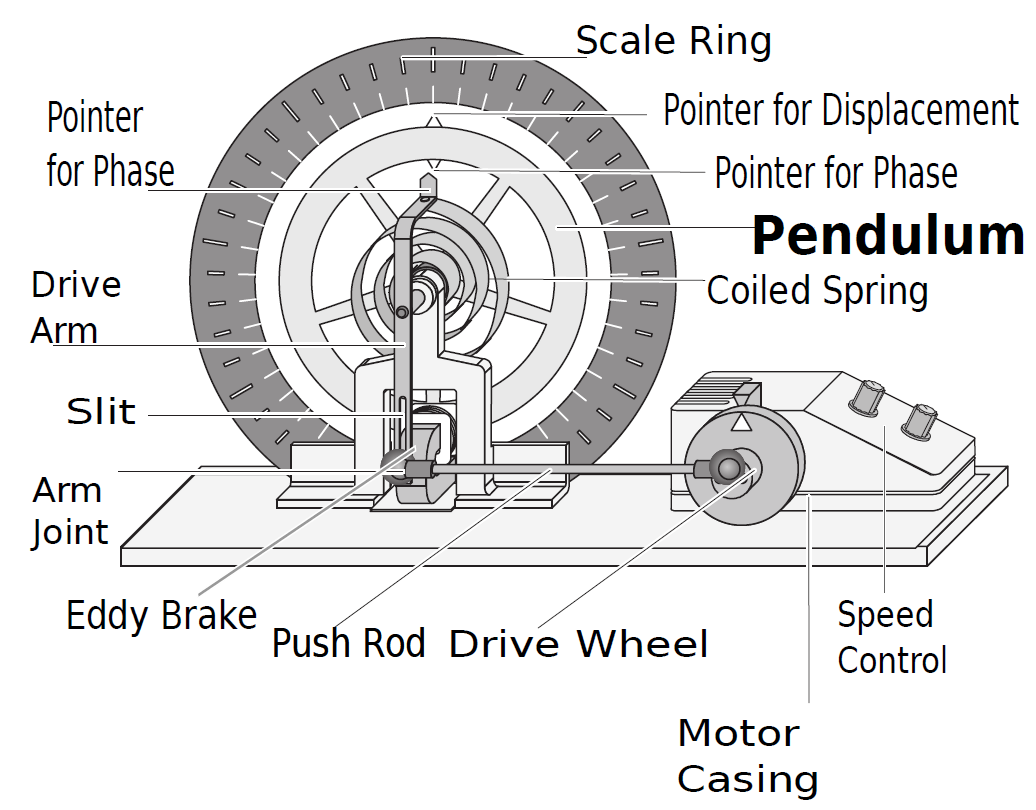
\includegraphics[width=0.5\linewidth]{images/pendulum_diagram.png}
\label{fig:system-diagram}
\end{figure}
Amplitude at $\omega = 0$ estimated to be $X(0) = \num{0.7 \pm 0.1}$.
\end{frame}



\begin{frame}{Forced oscillation}
\framesubtitle{Results}
Resonance frequency and the amplitude at resonance from the plot.
\begin{table}
   \centering
   \begin{tabular}{c c c}
   	\toprule
   	& $X_{max}$ & $\omega_{max} $\\
   	\midrule
   	$I_b=\num{0.3}\si{\ampere}$ & \num{11.5 \pm 0.1} & \num{3.11 \pm 0.02} \si{\per\second}\\
   	$I_b=\num{0.6}\si{\ampere}$ & \num{3.3 \pm 0.1} & \num{3.05 \pm 0.05} \si{\per\second}\\
   	\bottomrule
   \end{tabular}
   \label{table:resonance-results}
\end{table}
Thus, Quality factors are estimated to be:
   \begin{table}[H]\centering
   	\begin{tabular}{c c} 
   		\toprule
   		$Q^{2nd}$ [$I_b=0.3A$] & \num{16 \pm 2} \\
   		$Q^{2nd}$ [$I_b=0.6A$] & \num{4.7 \pm 0.7} \\
   		\bottomrule
   	\end{tabular}
   \end{table}
\end{frame}